\documentclass[12pt]{standalone}
\usepackage[utf8]{inputenc}
\usepackage[T1]{fontenc}
\usepackage{times}
\usepackage{amsmath,amssymb}
\usepackage[dvipsnames,svgnames]{xcolor}
\usepackage{tikz}
\usetikzlibrary{calc, positioning, arrows.meta}
\definecolor{winblue}{HTML}{0D366B}
\definecolor{inksec}{HTML}{52514E}
\definecolor{interf}{HTML}{C0504D}
% Adaptado de Marzetta et al. (2016), Fig. 2.7, p. 32: UEs nao-alvo na mesma celula (Zhao et al., Eq. 5).
\newcommand{\phone}[2]{%
  \begin{scope}[shift={#1}]
    \draw[line width=0.7pt, fill=#2, rounded corners=1pt] (-0.12,-0.22) rectangle (0.12,0.22);
    \draw[line width=0.7pt] (0.05,0.22) -- (0.05,0.31);
  \end{scope}}
\newcommand{\antena}[1]{%
  \begin{scope}[shift={#1}]
    \draw[line width=0.8pt] (0,0) -- (0.16,0);
    \draw[line width=0.8pt] (0.16,0) -- (0.29,0.09);
    \draw[line width=0.8pt] (0.16,0) -- (0.29,-0.09);
  \end{scope}}
\begin{document}
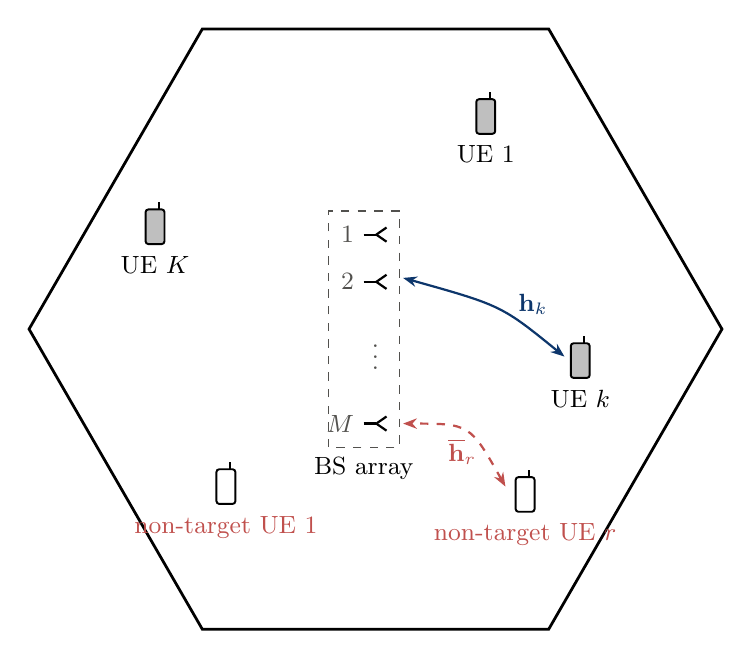
\begin{tikzpicture}[font=\fontsize{9}{10.8}\selectfont, >={Stealth[length=5pt]}]
% celula
\draw[line width=1pt] (0:4.4) -- (60:4.4) -- (120:4.4) -- (180:4.4) -- (240:4.4) -- (300:4.4) -- cycle;
% arranjo da BS
\foreach \y/\l in {1.2/1, 0.6/2, -1.2/M} {
  \antena{(-0.15,\y)}
  \node[inksec, left] at (-0.15,\y) {$\l$};
}
\node[inksec] at (0,-0.25) {$\vdots$};
\draw[dashed, inksec] (-0.6,-1.5) rectangle (0.3,1.5);
\node[below, align=center] at (-0.15,-1.5) {BS array};
% UEs alvo
\foreach \x/\y/\l in {1.4/2.7/1, 2.6/-0.4/k, -2.8/1.3/K} {
  \phone{(\x,\y)}{black!25}
  \node[below] at (\x,\y-0.25) {UE $\l$};
}
% UEs nao-alvo
\foreach \x/\y/\l in {-1.9/-2.0/1, 1.9/-2.1/r} {
  \phone{(\x,\y)}{white}
  \node[below, interf] at (\x,\y-0.25) {non-target UE $\l$};
}
% canais
\draw[<->, winblue, line width=0.8pt] (2.4,-0.35) .. controls (1.6,0.3) .. (0.35,0.65) node[pos=0.35, above right, inner sep=1pt] {$\mathbf h_k$};
\draw[<->, interf, dashed, line width=0.8pt] (1.65,-2.0) .. controls (1.2,-1.2) .. (0.35,-1.2) node[pos=0.55, below, inner sep=3pt] {$\overline{\mathbf h}_r$};
\end{tikzpicture}
\end{document}
